\chapter{Blockchain: Properties and Use Cases}

\begin{quote} \emph{"The Blockchain, initially used to solve problems in
  centralized financial systems, has inherent characteristics that, depending
  on the implementation, make it suitable for a variety of use cases. This
  Chapter will provide a more in-depth exploration of the Blockchain technology
  showing some of the considerations that were taken into account, after
  analyzing the alternative implementations previously mentioned in
  Chapter~\ref{background}, to choose the Hyperledger Fabric Distributed Ledger
  Platform to achieve the purpose mentioned in Chapter~\ref{introduction}.
  Finally some pratical implementations of Blockchain based solutions created
  to solve problems in the Healthcare field or problems managing entities are
  presented that provide context and show the current state of this technology
  in a production environment, providing an overview of both its shortcomings
  and successes thus far."} \end{quote}

\section{Trusting the Network}

Blockchain implementations are an emerging structure for distributed computing
systems, and provide an accurate and unchangeable history of transactions
written to a publicly available ledger or record, even when there is no trust
relationship between the parties involved~\cite{Barclay2017}.

Banks used to keep track of their financial transactions by writing on a book
called the ledger. The ledger would be written on when a new transaction
occurred, storing all details of the transaction that occurred between the bank
and other entities. Nowadays the ledger is not a book, instead being a
centralized database with the same function of recording all the transactions
that are made.

Imagine the following, Joe is on vacation and needs to borrow money from Jane,
his wife. Joe calls Jane to ask for some money and Jane tells him it will send
the money right away. Jane then proceeds to call her account manager in the
bank to transfer money to Joe. Finally Jane calls Joe to tell him the transfer
went through.  As seen on Figure~\ref{fig:centralizedvsdescentralized} Joe and
Jane need to use and trust the bank as a middle man in order to complete this
transaction. If the bank was ever to be unavailable, the database was corrupted
or if someone with  privileged access to the central database and malicious
intent was able to intercept the transactions from inside the bank then all
transactions between Joe and Jane would fail creating additional costs to all
parties involved. 

\begin{figure}[h]
  \centering
  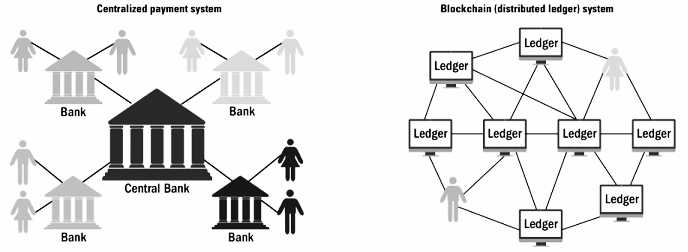
\includegraphics[width=1\linewidth]{imgs/blockchainvscentralizedNetwork.png}
  \caption{\label{fig:centralizedvsdescentralized} A comparison between a
  Centralized Banking System and a Distributed Ledger. (Source: Finance \&
  Development, 2016)}
\end{figure}

It was for a long time necessary, to establish trust between two entities, a
middle-man with a neutral stake in the transaction. While the ledger is also at
the core of the Blockchain, this technology aims to solve the dependency placed
upon third parties using decentralization and aims to make two different
entities trust each other through constant replication and through a process
called consensus.  Consensus is a mechanism that establishes a set of rules
that define if a chain of blocks is considered valid or not. In order to
properly explain how consensus works and why it is of such importance then
Blockchain network implementations must be categorized into two distinct
categories.

\section{Permissionless and Permissioned Networks}

As mentioned in this Chapter, Blockchain was created to solve problems that were
displayed in centralized financial systems. A centralized system is one that is
governed by a hierarchical authority; examples of such being banks, credit card
company’s, etc. If you want to use a Visa card you must request access from
Visa and be approved. At any time your access to that line of credit and your
funds may be made unavailable to you and your access permanently revoked
\cite{Dreifuerst2018}. The problem is that these centralized systems are
singular in number and therefore easily targetable.

In a decentralized network, participants work together to keep the network
corruption free. A decentralized network means that no single node can make a
decision individually, instead relying on other nodes to approve that change
and permanently add it to the record list. A decentralized network is a
subset of a distributed network.


%TODO

\section{Dealing with Identity Using Blockchain}
%TODO

\section{Blockchain Applied to Healthcare}

Some companies have already started developing Blockchain applications in the
Healthcare field and established some key partnerships.

Many Blockchain-based solutions are still very early on development or
deployment.  One exception is Guardtime, that has fully deployed their system
in 2008, started cooperating in 2011 and in 2016 announced a partnership with
the Estonian Government, where a million patient records are now secured by the
strategy and, until today, still proves the resilience of the Blockchain
technology, as well as, other advances in cryptography.  Now other companies
like Verizon are becoming interested in this technology for their own
purposes~\cite{GuardTime2018,EstonianGovernmentGuardTime2016}.

Another company, Gem, is collaborating with Phillips Healthcare to explore
options in this area, and is opting to solve the interoperability problem with
an additional layer of abstraction they call GemOS.  Factom, another
Blockchain-based service, has also announced a partnership with a major US
medical services provider
HealthNautica~\cite{BlockchainCompHealth2017,FactomPartnership2017}.

The use of the Blockchain technology in the health field is expanding. Just
recently a new platform appeared, called Medichain that allows patients to
store their own data in a secure way and give anonymized access to this data to
specialists. Giving data allows for users to gain tokens that represent
value~\cite{MediChain2018}.

\section{Hyperledger Fabric}
%TODO
